\chapter{Games with Team of Cooperative Agents}
\label{chap_mas}



In this chapter, we define perfect-information game in extensive form and perfect-information
game with teams in extensive form and discuss the coordination of agents and inter-agent
communication.


\section{Perfect-Information Game}


\label{sec_perfect_information_game}

This thesis deals with the problem of coordination of agents in games. Before we will review
work on this topic and propose our algorithms, it is necessary to define what the game in our
context is. We will consider finite, discrete, fully-observable, deterministic and static
environment in which we will talk about \emph{perfect-information game}. Following definition
is based on the definition
proposed in \cite{MAS2008} and generalized for our purposes (original definition does not
include posibility of simultaneous play of multiple players and forces a play of exactly one
player each turn).


\newtheorem*{defgpig}{Definition}
\begin{defgpig}[Perfect-information game]

A (finite) \textbf{perfect-information game} (in extensive form) is a tuple $G =
(P,A\cup\{\lambda\},S=S_n\cup S_p,\chi,\sigma,u)$, where:

\begin{itemize}

\item $P$ is a set of $n$ players;

\item $A$ is a (single) set of actions;

\item $S_n$ is a set of nonterminal choice states;

\item $S_t$ is a set of terminal states, disjoint from $S_n$;

\item $\chi: S_n \times P \mapsto 2^A \cup \{\lambda\} \setminus \varnothing$ is the action 
 function, which assigns to each choice node and player a set of possible actions, $\lambda \notin
 A$ is a neutral action played by the players not being on turn;

\item $\sigma: \{(s,a)| s \in S_n, a \in \prod\limits_{i\in P}\chi(s,i)\} \mapsto S$ is the
successor function, which maps a choice node and an action tuple to a new choice node or
terminal node such that for all $s_1, s_2 \in S_n$ and $a_1 \in \prod\limits_{i\in
P}\chi(s_1,i), a_2 \in \prod\limits_{i\in P}\chi(s_2,i)$, if 
$\sigma(s_1,a_1) = \sigma(s_2,a_2)$ then $s_1=s_2$ and $a_1=a_2$; and

\item $u = (u_1,\ldots,u_n)$, where $u_i: S_t \mapsto \mathbb{R}$ is a real-valued utility
function for player $i$ on the terminal nodes $S_t$.

\end{itemize}

We say that a perfect-information game is \textbf{turn-based} if each turn at most one player
plays an action, in other words, if the following restriction on the action function $\chi$ is satisfied:

\begin{equation}
\label{eq_turn_based_game}
\forall s \in S_n \; |\{i \in P|\chi(s,i) \not= \{\lambda\}\}| \le 1
\end{equation}

Note that our definition allows nodes with no player being on turn. This is reason why Equation
\ref{eq_turn_based_game} contains non-strict inequality.

Contrariwise we will call a perfect-information game \textbf{simultaneous} if simultaneous
plays of multiple players are permitted and a state forcing a play of at least two players
exists (and so Equation \ref{eq_turn_based_game} is not satisfied).

\end{defgpig}

Because we deal only with perfect-information games in our thesis, we will usually refer to
perfect-information game and its variants as to \emph{game}, \emph{turn-based game} and
\emph{simultaneous game}. We will also bound a utility function to $[0,1]$ (without loss of
generality).

The aim of a player $i$ is reaching a terminal node $s$ with the greatest possible utility
$u_i(s)$.

\subsection{Conversion between Turn-Based and Simultaneous Games}
\label{sec_turn_based_game_conversion}

Because a variant of MCTS used in this thesis requires turn-based games to ensure the
convergence (as discussed in
Section \ref{sec_minimax_convergence}) and our
algorithms, which are based on this specific MCTS variant, will be evaluated in the domain
of naturally simultaneous game,
we will need a conversion from a turn-based game to a simultaneous game, which will be described
here. Simultaneous nodes expansion modifies the game but our goal is not to develop the strongest 
possible players  for chosen domain but to study coordination algorithm related to MCTS and so
we choose retaining of algorithm properties.

We need to expand simultaneous actions to a sequence of single actions. To determine the order of such
an expansion, we can simply define linear ordering on a set of players. Then each simultaneous
action 
is splitted into multiple single-actions, one for each player, which is on turn.

There is, of course, a catch in this approach since the turn-based game created by this conversion
modifies game rules and adds advantage to players which plays later in originally simultaneous turn.
This is because players playing later have more information than in original simultaneous game
because they additionally know actions performed by players playing in same simultaneous turn.

In MCTS, when playing a simultaneous game, the calculated action will be commited to the simultaneous
game so the imbalance originating from the conversion will not affect the played game but only the
algorithm itself. We face the decision what ordering on players choose and we distinguish two main
variants - \emph{optimistic} and \emph{pesimistic expansion}. 

\begin{figure}
\begin{center}
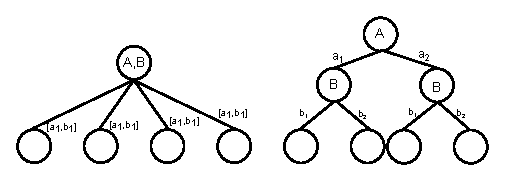
\includegraphics[width=12cm]{img/simultaneous_node_expansion.eps}
\end{center}
\caption{\footnotesize Simultaneous node expansion.}{\footnotesize Left - the node represents
simultaneous play of players $A$ and $B$ with sets of moves $\{a_1,_a2\}$ and $\{b_1,b_2\}$.
Right - expanded simultaneous node. Player $A$ is chosen to play first. If the player $A$ is an
owner of the tree, the expansion is pesimistic, otherwise, the expansion is optimistic.}
\label{fig_simultaneous_node_expansion}
\end{figure}

Optimistic expansion considers the
player performing MCTS calculation playing after all other players. This approach is called
optimistic because the player supposes that other players will play as he expect. On the other hand,
pesimistic expansion lets the player in MCTS calculations play first and gives other players
information about his action which is more pesimistic variant for the player. Expansion of
a simultaneous is ilustrated by Figure \ref{fig_simultaneous_node_expansion}.



\section{Team Coordination}

\subsection{Games with Teams of Players}
\label{sec_games_with_teams}

Definition of perferct-information game serves (without further modifications) as an
environment for \emph{teams of players}. A team of players (or simply a team) is a set of agents
attempting to reach the best result possible collectively. In other words, agents of a team
shares the utility function. 

This can be simply applied to a perfect-information game. A team can be represented as a single
player of a perfect-information game where actions of such a player is joint-action composed of
all actions played by team members. The second possibility how to model a team in
perfect-information game is adding teams as new entities in the game and considering players of
a single team sharing the same utility. Since it is more natural concept allowing the team 
player to be viewed as
independent agents, we will use this concept in our thesis. Following definition is a
formalization of the concept.


\newtheorem*{defpigt}{Definition}
\begin{defpigt}[Perfect-information game with teams]

A (finite) \textbf{perfect-information game with Teams} (in extensive form) is a tuple $G =
(P,A\cup\{\lambda\}, S=S_n\cup S_p, \chi, \sigma, T, \tau, u)$, where:


\begin{itemize}

\item $P$, $n$, $A$, $\lambda$, $S$, $S_n$, $S_t$, $\chi$ and $\sigma$ are same as in
perfect-information game;

\item $T$ is a set of teams;

\item $\tau: P \mapsto T$, assigns players to the teams; and

\item $u = (u_1,\ldots,u_m)$, where $u_i: S_t \mapsto \mathbb{R}$ is a real-valued utility
function for team $i$ on the terminal nodes $S_t$.

As in case of plain (without teams) perfect-information game, we distinguish turn-based and 
simultaneous game with teams of players. We say that game with teams is \textbf{turn-based} 
if only players of a same team play in all nodes. If we consider players of plain game being
members of virtual distinct teams, such a condition is generalization of plain turn-based game.
The condition is formalized by Equation \ref{eq_turn_based_game_with_teams}.

\begin{equation}
\label{eq_turn_based_game_with_teams}
\forall s \in S_n \; |\{t \in T|\exists i \in \tau^{-1}(t)\;\chi(s,i) \not= \{\lambda\}\}| \le 1
\end{equation}

Specially, we distinguish 
\textbf{pure turn-based game} with teams if only one player plays in each node (as requires
plain turn-based game without teams in Equation \ref{eq_turn_based_game}) and 
\textbf{weak turn-based game} not satisfying the condition. \textbf{Simultaneous game with
teams} is a game with teams not satisfying Equation \ref{eq_turn_based_game_with_teams}.


\end{itemize}

\end{defpigt}

A tuple of actions played by single team $T_a$ in state $S_b$ will be called \emph{joint-action} (formally
$(a_p^{S_b})_{\tau(p_a)=T_a}$).


\subsection{Distributed Constraints Optimization (??)}

\todo{?}


\subsection{Communication and Coordination}

Let us consider players of a team as defined in Section \ref{sec_games_with_teams}. Such
players share the utility function, attempting its maximization. The definifion of
perfect-information game with teams doesn't talk about the coordination, players are be viewed
as autonomous agents sharing no information about their intensions or reasoning. But sharing
such information is natural requirement for a team and is the way how to effectively coordinate
the players of the team.

Agents can share information by passing messages. In real-world applications, messages are
transmitted over a communication channel which has limited capacity and may be possibly
unreliable so it is necessary to consider length of message encoded to a particular form and.
These properties, in addition, force us considering the delay in transmission.

As an example of usage of message passing between independent agents is the distributed
constraint optimization problem \cite{Zivan2009}.
